\documentclass[article, 11pt, a4paper, onesize]{memoir}
\usepackage[article, serif, noindex]{ahsan}

\pagestyle{empty}
\title{\vspace{-3em}Final Project Review\vspace{-1em}}
\author{}


\begin{document}

\maketitle
\thispagestyle{empty}

\begin{minipage}[t]{.32\linewidth}
    M Ahsan Al Mahir\\
    ahsan.al.mahir@g.bracu.ac.bd\\
    20216007\\
\end{minipage}\hfill%
\begin{minipage}[t]{.38\linewidth}
    Atonu Roy Chowdhury\\
    atonu.roy.chowdhury@g.bracu.ac.bd\\
    20216008\\
\end{minipage}\hfill%
\begin{minipage}[t]{.29\linewidth}
    Ekram Wasi Shatil\\
    ekram.wasi.shatil@g.bracu.ac.bd\\
    16301072
\end{minipage}



\chapter{Abstract}

\subsection{Which system do you want to model?}

The system we modeled here is a Monte Carlo Simulation based on Percolation theory. It
deals with sales in Children's toy industry. This model tries to answer the question, "How
much quality should a product have in order to get x\% of the target customers?"

This system is modeled after the Social Percolation Model (Solomon et al. 2000).

\subsection{What do you want to simulate using this model?}

We wish to simulate the relation between the percolation threshold (product quality in
this case) and the ratio of the number of customers who buy the product and total target
customers.

\subsection{What questions will this simulation answer about the system?}

This simulation model will answer the following:

\begin{enumerate}
    \item Why do we experience sudden hits and flops in toy industry?
    \item How does the preference of parents and children effect a percolating system?
    \item What is a better percolating condition for social models? The spanning cluster
        method or the density method?
\end{enumerate}

\subsection{Why is this simulation important?}

This simulation is important to predict the system's behavior and take decisions
accordingly. Using this model with information from previous sales, companies can predict
the success rate of a given product.

\newpage
\chapter{Model Formulation}

\section{Write down the questions you asked to understand the system?}

\begin{enumerate}
\item What are the differences between the percolating model from the paper 'Social
    Percolation Models' and our model?  
\item How can we take both parents' and children's preferences into consideration?  
\item How should we take the weights parents give to their childrens' preferences into
    account?
\item If we take a weighted average of the preferences, should we set the weight 0.5 or we
    set thw weights at random?  
\item Is "existence of a spanning cluster implies hit" and "no spanning cluster implies
    flop" a really good metric to decide hit/flop?
\end{enumerate}



\section{Formulate the abstract model}

\subsection{What are the conditions of the experimental frame of this system?}

We consider parents and children to be cells in a square lattice. At first, a random set
of these cells are selected to be "agents". These agents have the knowledge of the
product, and can decide to buy it. 

Every cell has three numbers in \([0,1]\) assigned to it as the parents' preferences,
children's preferences and the weights on childrens' preferences. These numbers are
assigned randomly. The initial set of agents is chosen randomly. The change in
preference, \(dp\) for each children is the same.

\subsection{Define the system state variables, units and events.}

\begin{enumerate}
	\item The \(L\times L\) lattice is stored in a two dimensional array.
    \item Parent preferences \(p_i\) for each of the child on the lattice.
    \item Child preferences \(c_i\) for each of the child on the lattice.
    \item weight \(w_i\) that indicates how much child $i$'s preference is valued.
    \item The initial product quality \(q\)
	\item Number of agents
    \item The values \(dp\), \(dq\) that the dynamic model uses.
\end{enumerate}

\textbf{Events:}
\begin{enumerate}
	\item The agents are informed about the product.
    \item They buy the product if the product quality is higher than the weighted average
        of parent preference and child preference.
    \item If an agent buys the product, he will inform his neibouring lattices about the
        product. 
    \item Then the neighboring lattices become agents. A lattice that has already made a
        decision never becomes an agent again.
\end{enumerate}


\subsection{Explain the relationships between these system state variables and explain how
the variables change when events occur.}

\begin{enumerate}
    \item If an agent buys the product, that child's expectation rises up. So his
        preference index increases by \(dp\).
    \item Otherwise, that child's expectation goes down. So his preference index decreases
        by \(dp\).
    \item If the ratio (number of agents that buy the product)/(total number of agents) is
        greater than or equal to the desired ratio, then we will say the product is a hit.
        Otherwise we wil say the product is flop.
    \item If the product is a flop, the quality \(q\) needs to be increased. If the
        product is hit, the quality \(q\) needs to be decreased to ensure optimal profit.
        In each of the cases, \(q\) increases or decreases by \(dq\).
\end{enumerate}


\subsection{Using the above answers define the Mathematical Model for this system.}

\begin{enumerate}
    \item Total number of agents is \(L^2\). An agent's decision is denoted by \(d=c\times
        w+p\times(1-w)\), where \(c,p,w\) are child preference, parent preference, weight
        respectively. 
    \item If \(q>d\), the agent will buy the product, that agent's neighbor's will be
        agents, and \(c=c+dp\) for that agent.
    \item If \(q<d\), the agent doesn't buy the product, and \(c=c-dp\) for that agent. 
    \item We shall continue this for all the agents. Then check if the product is hit or
        flop for that particular \(q\). 
    \item If the product is hit, \(q=q-dq\). If the product is flop \(q=q+dq\). Then we
        shall continue the whole process. Here the 2D arrays denoting parents'
        preferences, children's preferences and weights - all are generated randomly.
\end{enumerate}


\subsection{What percentage of your model can you implement? (Which parts of your model
can you implement) Justify your expectation.}

The model uses very basic concepts of percolation theory. So we think the model is easily
implementable.


\subsection{What percentage of the simulation can be done using your expected model
implementation? Justify.}

The model implementation is expected to simulate the whole simulation, except validation.
Because we do not have access to a reliable data set with which we can compare the
simulation result.


\subsection{The papers you read to formulate the model of your system should be referred
within the document.}

``Social Percolation Models", writers: Solomon, S., Weisbuch, G., Arcangelis, L., Jan, N.,
Stauffer, D (2000).

URL: \url{https://www.sciencedirect.com/science/article/abs/pii/S0378437199005439}


\newpage
\chapter{Implementation and Output Analysis}

\section{Implementation of the Model}

\subsection{Which simulation techniques (names of numerical methods, modern techniques)
will you need to simulate the system?} 

We used Monte Carlo Simulation for producing our data. We used the ideas from
Percolation theory for social models. We didn't require any numeric analysis
methods.

\subsection{Describe the organization of your program.}

Our program uses a system class that holds all the system state variables and methods. We
have the following methods:

\begin{lstlisting}[style=mypy]
class system: # main class
    variables:
        q        # initial product quality
        r        # we say system is percolating if r*L*L people purchased
        parents  # array for parents preferences
        children # array for children preferences
        weights  # array for weights
        agents   # stores the current agents
        dp, dq   # increment values

    gen_agents()     # generates random agents at the start of a phase
    neighbors()      # helper function to return the neighbors of a lattice cell
    decision()       # returns the decision for a cell
    is_percolating() # checks whether the system is percolating or not
    increment_time() # runs a full simulation of all the lattices
    increment_vals() # changes the values using dp and dp
\end{lstlisting}

We store the values \(p_i, c_i, w_i\) in arrays named \texttt{parents, children, weights}.
When we increment time, that is when we evaluate the change for a product, we first create
a random set of agents using \texttt{gen\textunderscore agents()} method. We then create a
\texttt{blacklist} array to keep track of all the people who made a decision about this
product. We also create a \texttt{purchased} array to list those who bought the product. 

After the time increment, we change the values of \(c_i\) and \(q\) following the
criterions. Then we run the same simulation again.


\subsection{Update your codes}

The code can be found at \url{https://github.com/AnglyPascal/cse474_final_project/}

\section{Result Analysis}

The final value of \(q\) converges regardless of weights and parents'- childrens' preferences.
The following graph shows the convergence for \(r=.5, L=100, q=.575, dq=1e-4\) for ten random systems.

\begin{center}
    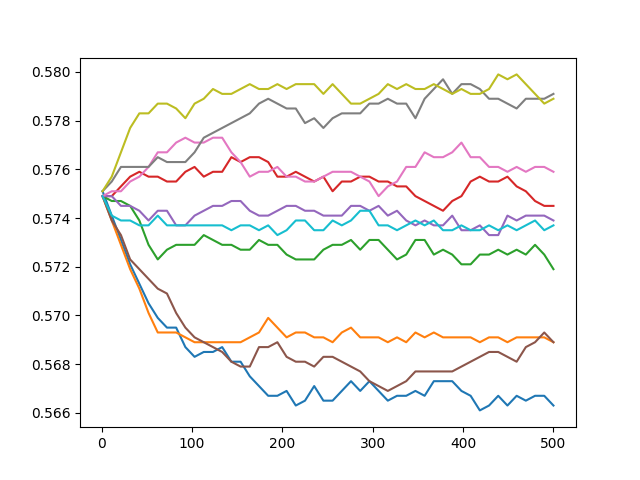
\includegraphics[scale=0.6]{q_converges_L100_q575_r5_num10_dq1e-4.png}

    This figure shows the convergence of \(q\) as time increases in \(10\) lattices
    of size \(100\times 100\) with starting value of \(q=.575\).
\end{center}

\begin{center}
    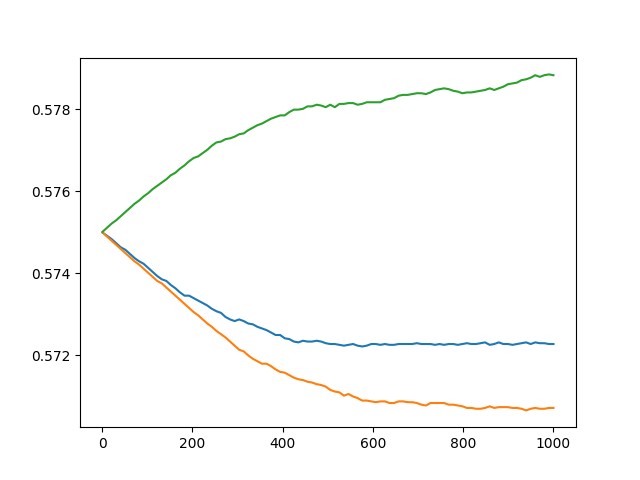
\includegraphics[scale=0.6]{q_converges_L200_q575_r5_num3_dq1e-5.png}

    This figure shows the convergence for \(3\) random lattices of size \(200\times 200\)
    with values \(r=.5, q=.57, dq = 1e-4\)
\end{center}

In the following graph, we see how the value of \(q\) evolves with our definition of
percolation based on density. As the value of \(r\) goes from \(0\) to \(q\), the value of
\(q\) increases from \(.4\) to \(1\).

\begin{minipage}{.5\linewidth}
    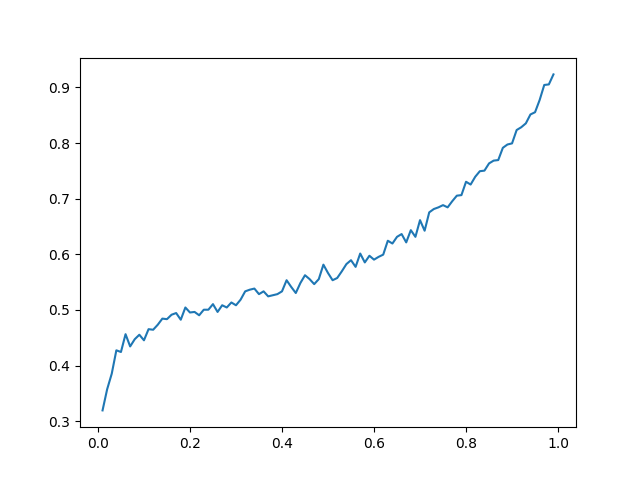
\includegraphics[width=.9\linewidth]{ratio_vs_qqq.png}

    \begin{center}
        \(L=100\), for \(100\) values of \(r\)
    \end{center}
\end{minipage}\hfill%
\begin{minipage}{.5\linewidth}
    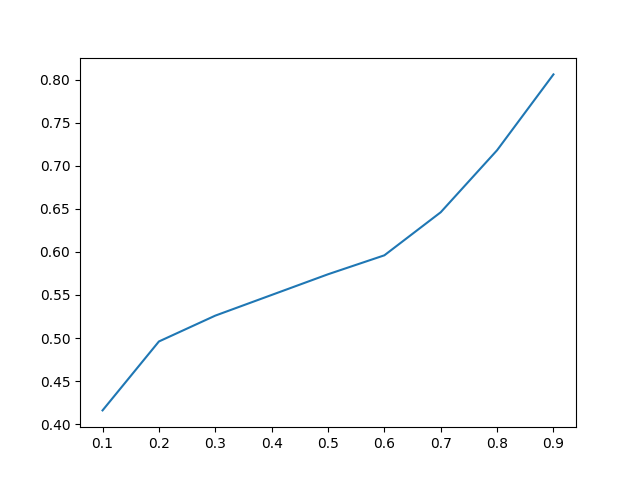
\includegraphics[width=.9\linewidth]{ratio_vs_qq.png}

    \begin{center}
        \(L=200\), for \(10\) values of \(r\)
    \end{center}
\end{minipage}



\section{Validation and Verification}

\textbf{Verification:}

Our model accurately reflects our conceptual model. During our model development, we found
that if we used the spanning cluster method for determining whether the product quality
should increase or not, our system behave wildly. Instead if we used the density method,
we can predict the behavior of the system. It also reflects the real life scenario more
accurately, since industries collect their data statistically. 

Since our output also reflects the fact that for some products with quality less than our
predicted threshold, then it can be classified as a flop, and that prepresents the real
life phenomena.

\textbf{Validation}:

We can't yet validate our model, since we don't have the real life data. But with access
to the data from market, our model can be easily validated.




\section{Self Assessment}

Our model could be further improved by taking the following factors into account:

\begin{enumerate}
    \item Children's social environment, i.e. their schools and neighbors, and the
        interactinos between them and their friends.
    \item Multiple sibling scenarios
    \item Children's age factor
\end{enumerate}




\end{document}
